Este capítulo é dedicado à implementação do primeiro algoritmo de \textit{Data Augmentation}, onde são geradas RIRs simuladas (RIRSM)
a partir de RIRs originais (RIRO), que foram gravadas em ambientes diversos e compõem o banco de dados AIR \cite{AIR_Database}. 
São observados os parâmetros de razão Direto-Reverberante (DRR) e tempo de reverberação (T60), que são
inferidos com base em uma RIRO e que serão manipulados pelo algoritmo para gerar RIRs que vão representar modelos acústicos diferentes.

\begin{figure} [H]
    \centering
    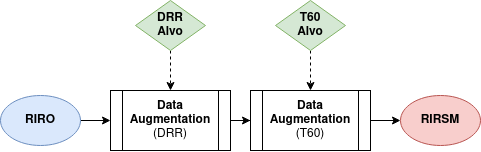
\includegraphics[scale=0.6]{flow-rir-aug.png}
    \caption{Fluxo de procedimentos para gerar a RIRSM.}
    \label{fig:flow-rir-aug}
\end{figure}

Este trabalho é uma implementação dos passos demonstrados no artigo \cite{RIR_Data_Aug}. A Figura \ref{fig:flow-rir-aug} especifica 
o fluxo de procedimentos implantados por este algoritmo, onde a DRR e T60 alvos são os valores escolhidos pelo usuário ou sorteados aleatoriamente,
que determinam as características da RIRSM. 

Antes de explicar os métodos usados, é necessário definir duas funções \cite{RIR_Data_Aug}:

\begin{align} 
    h_e(t) &= 
    \begin{cases} \label{eqn:rir-early}
        h(t), & t_d-t_0 \le t \le t_d+t_0 \\
        0, & \text{caso contrário,}
    \end{cases} \\
    h_l(t) &= 
    \begin{cases} \label{eqn:rir-late}
        h(t), & t < t_d - t_0 \\
        h(t), & t > t_d + t_0 \\
        0, & \text{caso contrário,}
    \end{cases}
\end{align}

\noindent
onde $t$ representa o tempo discreto, $t_d$ o tempo que as ondas sonoras diretas, ou seja, sem reflexão, levam da fonte até o destino de gravação,
$t_0$ a janela de tolerância, neste caso definida com o valor 2,5 ms \cite{RIR_Data_Aug}, 
$h(t)$ uma RIR, $h_e(t)$ as primeiras reflexões e $h_l(t)$ as reflexões tardias.
Neste algoritmo, $t_d$ é determinado da forma:

\begin{align} \label{eqn:t_d}
    %t_d = t_{max},\ onde \ \ h(t_{max}) = max(h(t))
    \begin{cases}
        t_d = t_{max},\\
        t_{max}, \ \text{onde} \ h(t_{max}) = max(|h(t)|)
    \end{cases}
    .
\end{align}


\section{Razão Direto-Reverberante (DRR)}


A DRR representa a razão entre a energia sonora da resposta ao impulso que atinge o alvo diretamente e a energia reverberante,
ou seja, que é refletida pelas paredes do ambiente fechado. Este parâmetro é calculado pela seguinte expressão:

\begin{equation} \label{eqn:DRR_def}
    DRR_{dB} = 10 \log_{10} \left( \frac{\sum_t h^2_e(t)}{\sum_t h^2_l(t)} \right).
\end{equation}

Para obter a $DRR_{dB}$ alvo desejada, aplica-se um fator de ganho escalar $\alpha$ na função das primeiras reflexões $h_e(t)$.
De acordo com \cite{RIR_Data_Aug}, para evitar descontinuidades durante o cálculo do fator $\alpha$, reescreve-se 
$h_e(t)$ em duas parcelas, uma que representa a janela direta no pico de intensidade de $h(t)$ e outra
que representa uma janela de resíduo de $h_e(t)$ formando, assim,

\begin{equation} \label{eqn:new-h_e}
    h'_e(t) = \alpha w_d(t) h_e(t) + [1 - w_d(t)]h_e(t),
\end{equation}

\noindent
onde $w_d(t)$ representa uma janela de Hann de duração de 5 ms, considerando-se uma janela de tolerância $t_0 = 2,5$ ms.
Substituindo na Equação (\ref{eqn:DRR_def}) $h_e(t)$ por $h'_e(t)$ e combinando com a Equação (\ref{eqn:new-h_e}), obtém-se
a seguinte equação quadrática;

\begin{equation} \label{eqn:DRR_quad_eqn}
    \begin{aligned} 
        \alpha^2 \sum_t w^2_d(t) h^2_e(t) +
        2 \alpha \sum_t [1 - w_d(t)] w_d(t) h^2_e(t) + \\
        \sum_t [1 - w_d(t)]^2 h^2_e(t) -
        10^{DRR_{dB}/10} \sum_t h^2_l(t)
        = 0 ,
    \end{aligned}
\end{equation}

O parâmetro $\alpha$ desejado será a raiz de maior valor. 
Uma ressalva deste procedimento é que se deve atentar para não escolher uma $DRR_{dB}$ que não seja muito menor que a original,
pois após a transformação de $h_e(t)$ para $h'_e(t)$, dependendo do valor de $\alpha$, é possível incidir em um caso onde
$max(h'_e(t)) < max(h_l(t))$, tornando a RIRSM impraticável.

A Figura \ref{fig:ir-early} exibe um exemplo de sinal $h(t)$ com o seu $h_e(t)$ após ser feita a modificação do DRR.
Comparando $h_e(t)$ com $h'_e(t)$, de acordo com a Figura \ref{fig:drr-da}, nota-se que $h'_e(t)$  está com uma intensidade 
maior, o que condiz a modificação do DRR de -4,5 dB para 4 dB neste exemplo.

\begin{figure}[H]
    \centering
    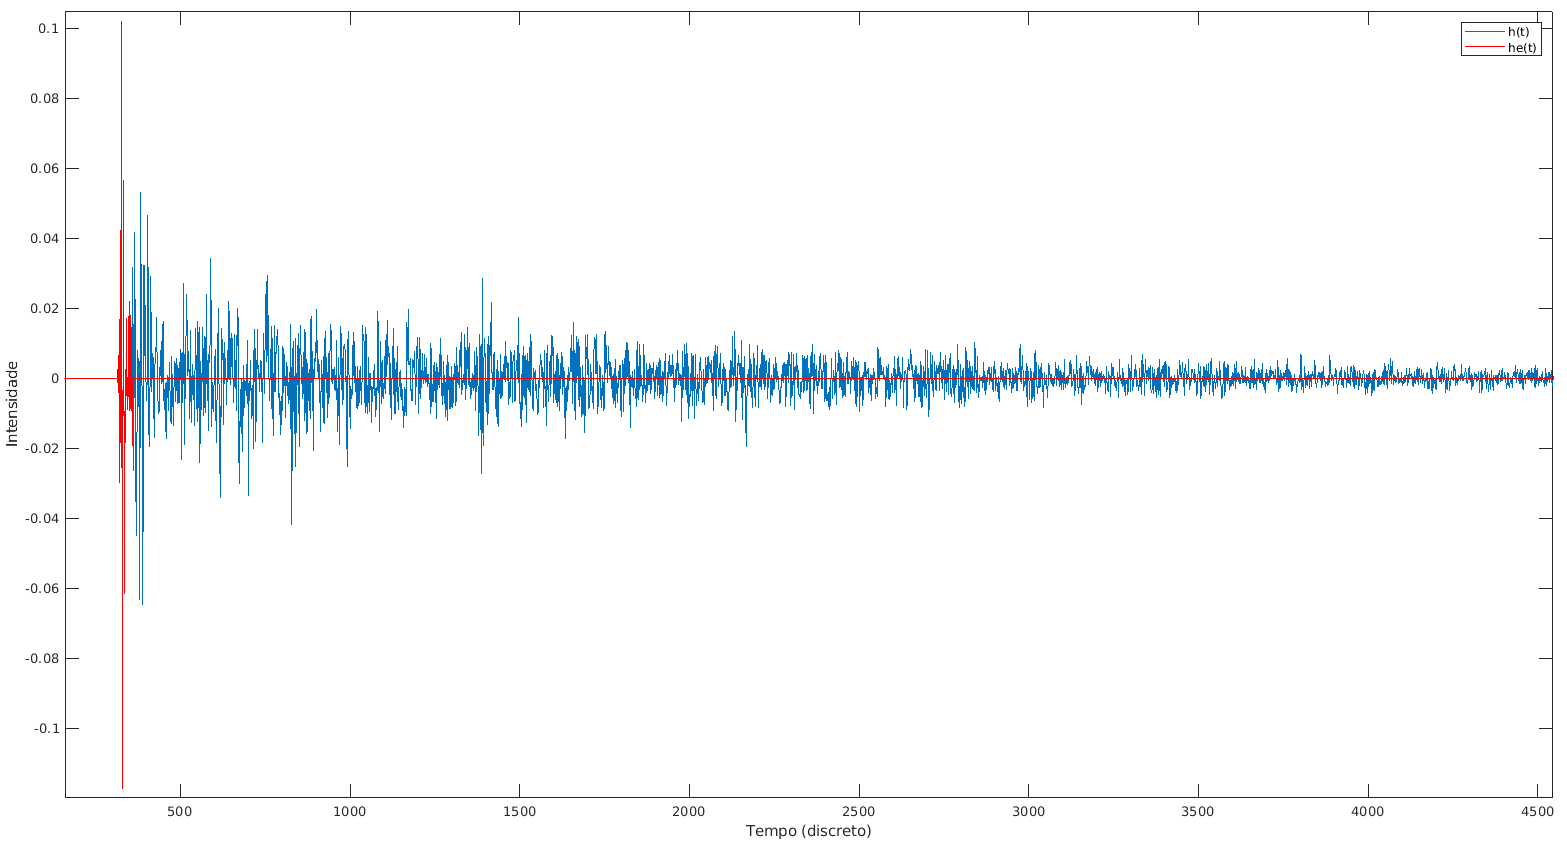
\includegraphics[scale=0.3]{ir-early.png}
    \caption{Um exemplo de $h(t)$ com $h_e(t)$, onde é feita a modificação do DRR de -4,5 para 4, marcado em vermelho.}
    \label{fig:ir-early}
\end{figure} 

\begin{figure}[H]
    \centering
    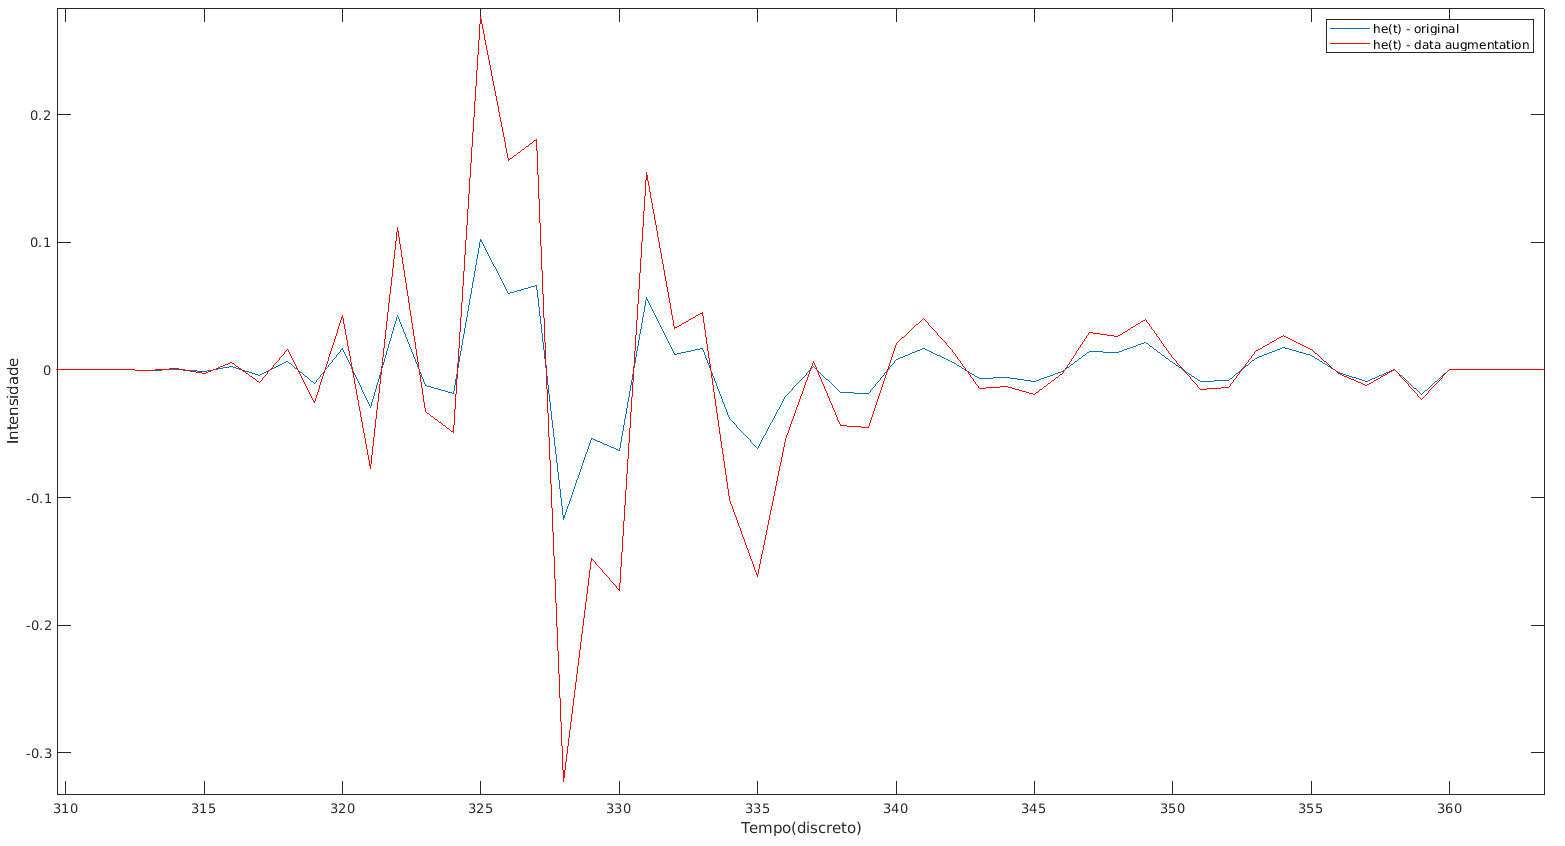
\includegraphics[scale=0.3]{drr-da.png}
    \caption{Um exemplo de $h_e(t)$ antes e depois da aplicação do algoritmo, original em azul ($DRR=-4,5$ dB) e o modificado em vermelho ($DRR=4$ dB).}
    \label{fig:drr-da}
\end{figure} 


\section{Tempo de Reverberação (T60)}


O T60, definido na equação \ref{eqn:T60-def}, representa a duração de tempo que leva para a energia sonora da RIR
no alvo decair 60 dB comparado à sua intensidade máxima. Geralmente, devido à dificuldade de se medir uma queda de 60 dB,
o parâmetro medido é o T20 ou o T30 e depois multiplica-se os seus valores por 3 e 2, respectivamente, para obter o T60,
assumindo-se um decaimento exponencial da envoltória da RIR.

\begin{align} \label{eqn:T60-def}
    \begin{cases}
        \text{T60} = t_f-t_i, \ \text{onde}\\
        t_i \rightarrow h(t_i) = max(h(t)) \\
        t_f \rightarrow 10 \log_{10} \left( h^2(t_i) - h^2(t_f) \right) = 60 \text{dB} \\
        %t_i, \ \text{onde} \ h(t_i) = max(h(t)) \\
        %t_f, \ \text{onde} \ 10 \log_{10} \left( h^2(t_i) - h^2(t_f) \right) = 60 \text{dB} \\
        %\text{T60} = t_f-t_i.
    \end{cases}
    .
\end{align}

Para realizar modificações na RIR, é necessário modelar a função das reflexões tardias. De acordo com \cite{RIR_Data_Aug},
um modelo normalmente usado é de um ruído gaussiano exponencialmente decadente, acrescido de um ruído residual, ou seja,

\begin{equation} \label{eqn:h_l-gauss}
    h_m(t) = A e^{-(t - t_o)/ \tau} n(t) u(t - t_o) + \sigma n(t)
    ,
\end{equation}

\noindent
onde $A$ representa o ganho da resposta ao impulso, $\tau$ a taxa de decaimento, $\sigma_m$ o desvio padrão do ruído residual, 
$n(t)$ um ruído gaussiano padrão (média nula e desvio padrão unitário), $t_o$ o valor temporal onde $h_l(t)$
tem o seu primeiro valor não nulo e $u(t)$ um degrau unitário.
Neste trabalho, diferente da implementação do algoritmo em \cite{RIR_Data_Aug}, é considerada apenas a taxa de decaimento
do espectro de frequência por completo da RIR, ao invés de dividi-la em subbandas e analisar 
a taxa de decaimento para cada faixa de frequência.

Os parâmetros $A$, $\tau$ e $\sigma$ são estimados de acordo com o padrão definido na ISO 3382-1 \cite{ISO-3382}.
Seja $T60_d$ o valor de T60 alvo para DA, é possível inferir a taxa de decaimento através da equação

\begin{equation} \label{eqn:decay-rate-t60}
    T60_d = \ln(1000) \tau_d T_s
    ,
\end{equation}

\noindent
onde $\tau_d$ representa a taxa de decaimento alvo e $T_s$ o intervalo de amostragem.
A DA do tempo de reverberação é feita multiplicando-se $h_l(t)$ pela exponencial

\begin{equation} \label{eqn:DA-T60}
    h'_l(t) = h_l(t) e^{-(t - t_o) \frac{\tau - \tau_d}{ \tau \tau_d} }
    .
\end{equation}

Por fim, a RIRSM completa, $h'(t)$, pode ser representada pela equação

\begin{equation} \label{eqn:RIRSM}
    h'(t) = h'_e(t) + h'_l(t)
    .
\end{equation}

A Figura \ref{fig:ir-late} exibe um exemplo de sinal $h(t)$ com o seu $h_l(t)$ após ser feita a modificação do T60.
Comparando $h_l(t)$ com $h'_l(t)$, de acordo com a Figura \ref{fig:t60-da}, nota-se que $h'_l(t)$  está com uma intensidade 
maior, o que condiz a modificação do T60 de 1,38 para 2,6 segundos neste exemplo.

\begin{figure}[H]
    \centering
    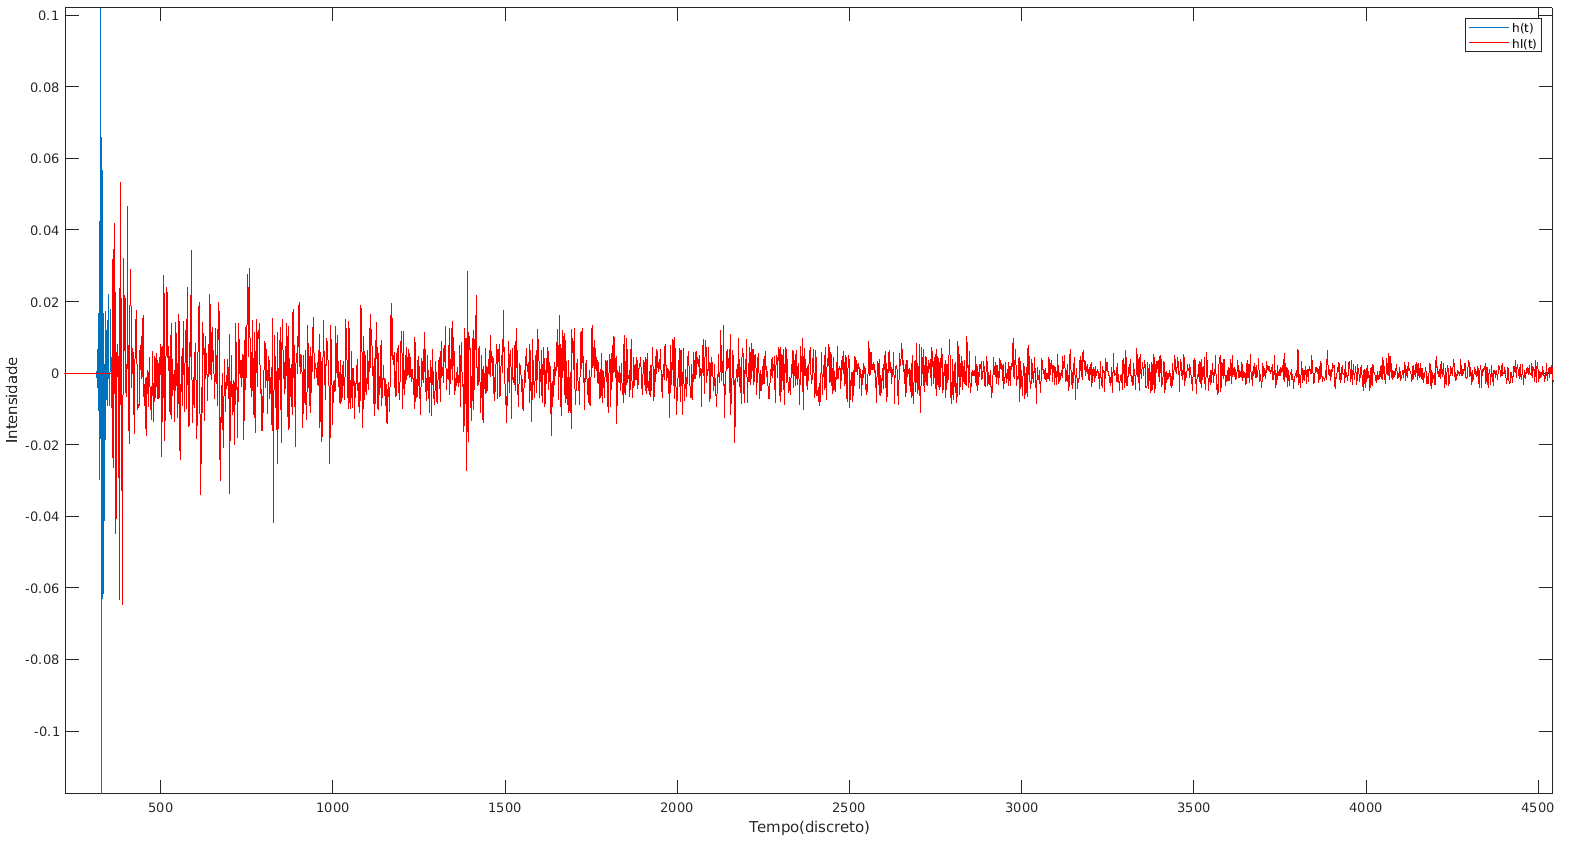
\includegraphics[scale=0.3]{ir-late.png}
    \caption{Um exemplo de $h(t)$ com $h_l(t)$, onde é feita a modificação do T60 de 1,38 para 2,6 segundos, marcado em vermelho.}
    \label{fig:ir-late}
\end{figure} 

\begin{figure}[H]
    \centering
    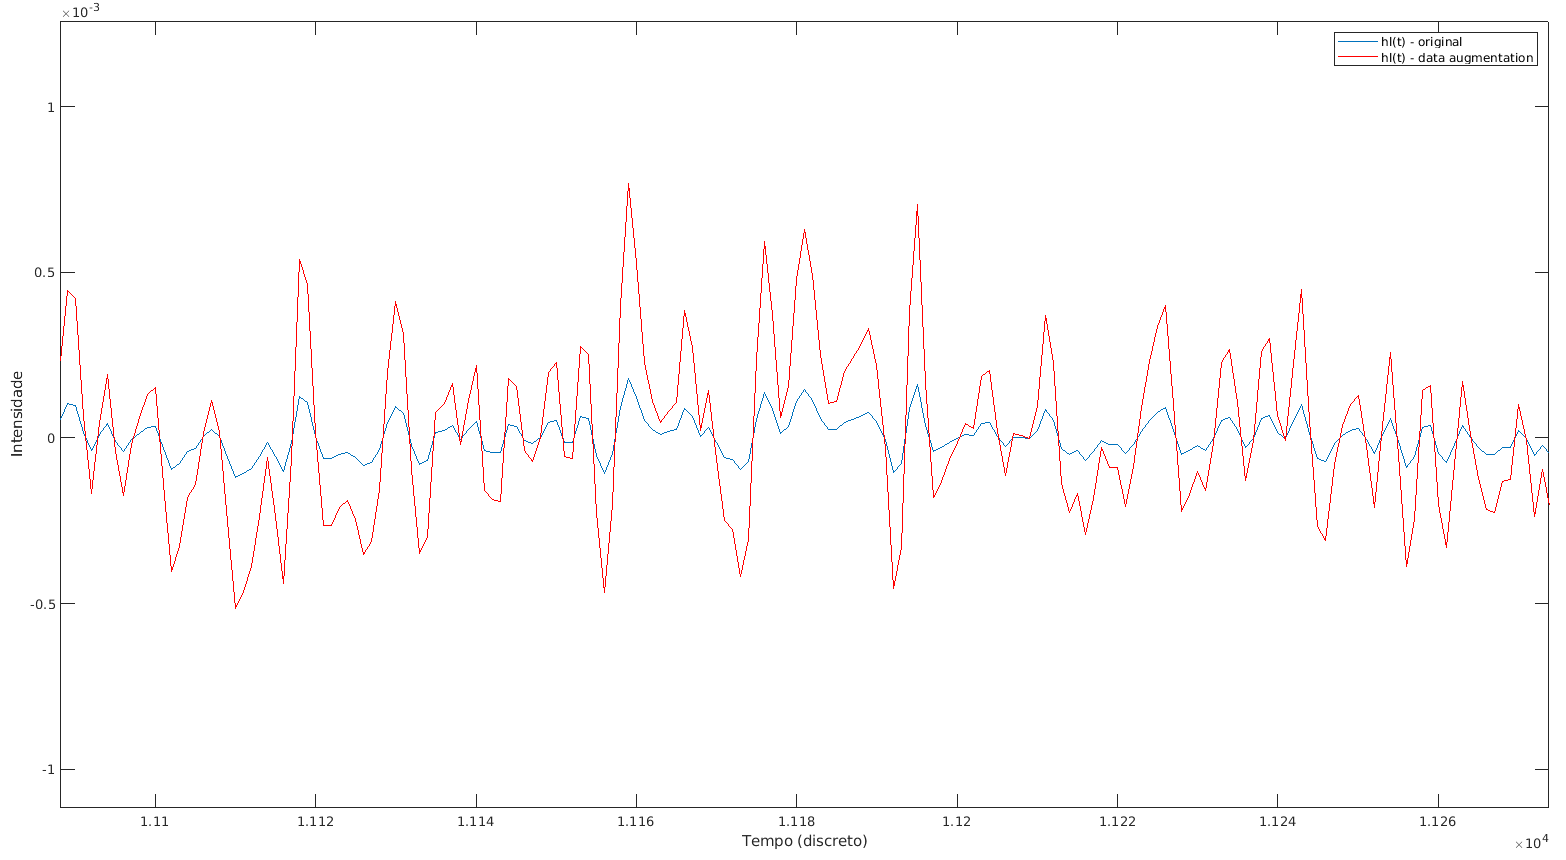
\includegraphics[scale=0.3]{t60-da.png}
    \caption{Um exemplo de um trecho ao final de $h_l(t)$ antes e depois da aplicação do algoritmo, original em azul ($T60=1,38$ s) e o modificado em vermelho ($T60=2,6$ s).}
    \label{fig:t60-da}
\end{figure} 